% ****** Start of file apssamp.tex ******
%
%   This file is part of the APS files in the REVTeX 4.2 distribution.
%   Version 4.2a of REVTeX, December 2014
%
%   Copyright (c) 2014 The American Physical Society.
%
%   See the REVTeX 4 README file for restrictions and more information.
%
% TeX'ing this file requires that you have AMS-LaTeX 2.0 installed
% as well as the rest of the prerequisites for REVTeX 4.2
%
% See the REVTeX 4 README file
% It also requires running BibTeX. The commands are as follows:
%
%  1)  latex apssamp.tex
%  2)  bibtex apssamp
%  3)  latex apssamp.tex
%  4)  latex apssamp.tex
%
\documentclass[%
 reprint,
%superscriptaddress,
%groupedaddress,
%unsortedaddress,
%runinaddress,
%frontmatterverbose, 
%preprint,
%preprintnumbers,
%nofootinbib,
%nobibnotes,
%bibnotes,
 amsmath,amssymb,
 aps,
%pra,
%prb,
%rmp,
%prstab,
%prstper,
%floatfix,
]{revtex4-2}

\usepackage{graphicx}% Include figure files
\usepackage{dcolumn}% Align table columns on decimal point
\usepackage{bm}% bold math
\usepackage{commath}
\usepackage[hidelinks]{hyperref}
\usepackage{cleveref}
\usepackage{float}
\usepackage{lipsum}

% \usepackage{wrapfig}
% \usepackage[font=small,labelfont=bf]{caption}
% \usepackage{subcaption}
% \usepackage{color}
% \usepackage{listings}
% \usepackage{tabularx}
\usepackage{svg}
% \usepackage{mhchem}
\usepackage{tikz}
\usetikzlibrary{matrix, positioning}

%\usepackage[mathlines]{lineno}% Enable numbering of text and display math
%\linenumbers\relax % Commence numbering lines

% \usepackage[showframe,%Uncomment any one of the following lines to test 
%%scale=0.7, marginratio={1:1, 2:3}, ignoreall,% default settings
%%text={7in,10in},centering,
%%margin=1.5in,
%%total={6.5in,8.75in}, top=1.2in, left=0.9in, includefoot,
%%height=10in,a5paper,hmargin={3cm,0.8in},
%]{geometry}

\begin{document}

\preprint{APS/123-QED}

\title{Percolation Theory:\\an Investigation}% Force line breaks with \\

\author{Oliver Dudgeon}
\author{Adam Shaw}
\author{Joseph Parker}

\date{\today}

\begin{abstract}
\lipsum[1]
\end{abstract}

%\keywords{Suggested keywords}%Use showkeys class option if keyword
                              %display desired
\maketitle

\section{Introduction}

\begin{figure}
    \centering
    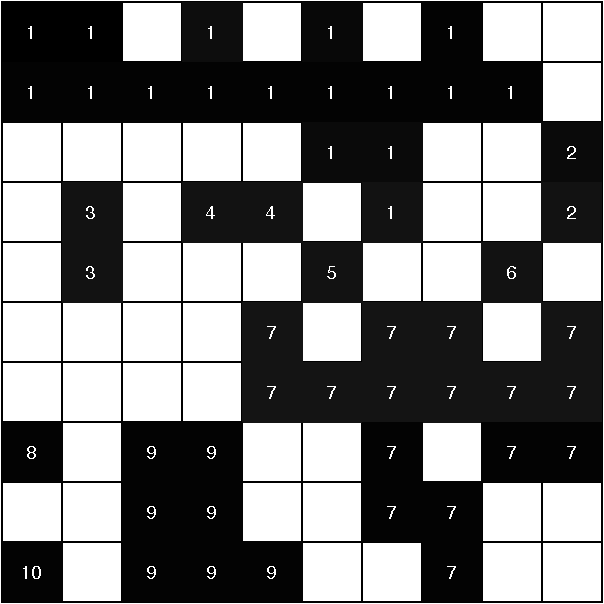
\includegraphics[width=0.7\linewidth]{report/assets/grid.pdf}
    \caption{A 10 by 10 square lattice. Occupied sites are filled. The number in each site corresponds to the cluster the site is a member of. }
    \label{fig:2D_lat}
\end{figure}

In percolation theory a number of objects are randomly placed with a probability $p$. Sometimes, these objects are connected by their nearest neighbours. The objects can then be divided into clusters. Each object belongs to one cluster. Each cluster has one or more objects. One representation of this is that of the two-dimensional square lattice like in \cref{fig:2D_lat}. 

Percolation theory handles the properties of these clusters. It is often useful to analyse the number of clusters, the sizes of clusters and the shapes of clusters. It is also possible that a cluster spans the entire space. This means there is a cluster for which one can construct a path from one side of the grid to the opposite side of the grid without leaving the original cluster. 

Although at first glance this can seem like a mathematical interest with not much practical use, this model is used in the study of statistical mechanics including the Ising model; disorder in superconductors \cite{alexander_superconductivity_1983}; traffic networks \cite{li_percolation_2015} and epidemic modelling including the COVID-19 pandemic \cite{mello_epidemics_2020}.

In this article we restrict ourselves to the two-dimensional square lattice, however, there are many other possible layouts used in percolation theory such as higher dimension site percolation and bond percolation where instead of filling a cell on a grid a link between two sites is made. This bond has six nearest neighbours where the 2D site model has just four. 

The article is structured as follows. First we develop the methods of two models. Firstly, \cref{sec:site} describes a model of site percolation on a 2D lattice and secondly, \cref{sec:ff} describes a model of forest fires. 

% \subsection{Structure}

% \begin{itemize}
%     \item Generic description of perc theory \cite{stauffer_introduction_2003} y
%     \item Site and Bond percolation y
%     \item Areas where it's used y
%     \begin{itemize}
%         \item Epidemic models (COVID-19) \cite{mello_epidemics_2020} y
%         \item Ising model --- Magnetic systems y
%         \item disorder in superconductors  y
%         \item diluted magnetic semiconductors
%         \item traffic network y
%     \end{itemize}
%     \item Why investigate further
%     \item Report structure
% \end{itemize}

\section{Models}\label{sec:models}
\subsection{Site percolation on a 2D lattice}\label{sec:site}
For a 2D lattice, where sites are filled with a probability $p$, there exists a critical probability at which you are more likely to find a infinite cluster than you are to not find one. Around this point there are few properties that we can explore, such as phase change and critical exponents that describe the asymptotic behaviour.

To generate these grids for our chosen probability $p$, for each site, we generate a random number between 0 and 1. We then check if this number is less than $p$, if it is we fill the site i.e. set it to 1 in an array (0 would mean empty).

The critical value $p_{c}$ has different meanings for infinite and finite grids. For infinite grids past $p_{c}$ you will defiantly see an infinite cluster appearing. For finite grids above $p_{c}$ you are more likely to find a grid where the sites connect two sides than one where they don't.

To analyse the properties of these cluster we would like to know which sites belong to which cluster, from this we can extract the rest of the information about the grid we want. Two sites are said to be connected when they share a common edge, this restricts each site to having 4 neighbours. Knowing this allows to use an algorithm called the Hoshen-Kopelman algorithm \cite{hoshen_percolation_1976} (HK algorithm), which is very efficient as it only requires two passes over the grid. On the first run it checks the left and top neighbour of each site going from left to right then top the bottom. If there are no neighbours then a new cluster is created, for one neighbour then it will already be in a cluster so assign the current site that cluster. Finally for two cluster they will both already have cluster numbers, which are not necessarily the same hence we need to link them together. After all this is done, we go over the array again linking all the clusters together so that they have incremental labels. The algorithm is outline in this flow chart\cref{fig:hk_flow}. Running the HK on the grid in \cref{fig:2D_lat} gives you the labels that are present in the figure.

\begin{figure}[H]
    \centering
    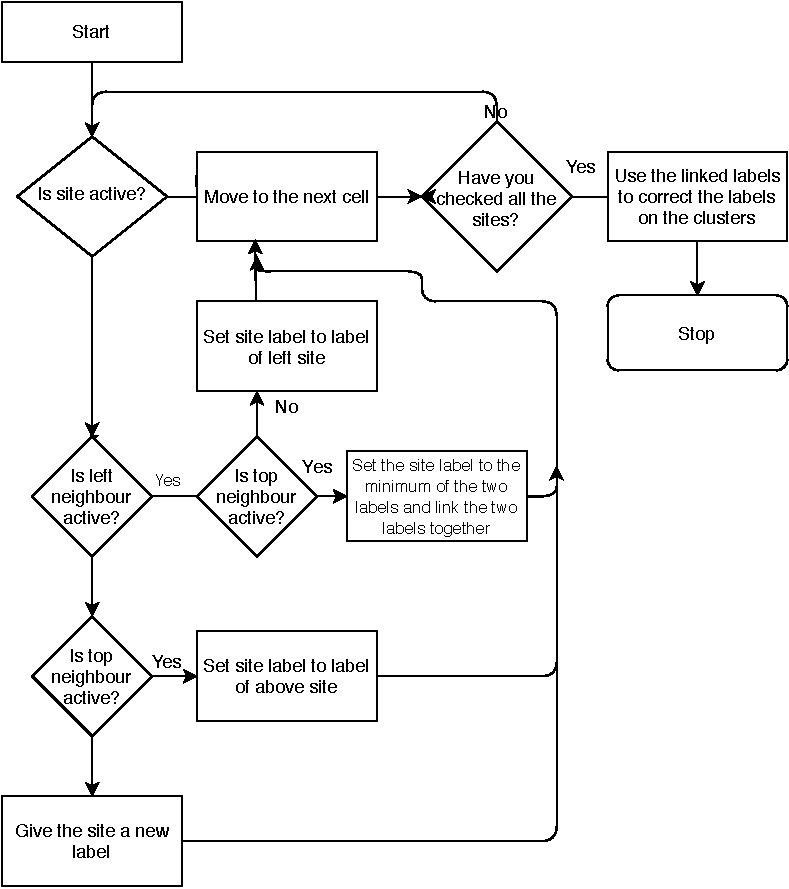
\includegraphics[width=\linewidth]{report/assets/hk_algroithm.pdf}
    \caption{Hoshen-Kopelman algorithm flow chart. This iterates through the sites labelling each site with the cluster it belongs to. }
    \label{fig:hk_flow}
\end{figure}

For our results we decided to try and optimise this algorithm by making use of multiple processing cores. To do this we chose to run the HK algorithm on a different grid for each core. This limited the size of our grids as running multiple at once uses a lot of memory. It did decrease the time it took for our programs by about x30. Normally you would want to run a bigger grid, in this case you would split up the grid into smaller sub grids then run each sub grid on a separate processor. Once they've all done, you recombine them again into the bigger grid. Using this allows you to analyse far greater grid sizes.

For our program we ended up not using this algorithm, but rather chose a newer algorithm implemented in SciPy's ndimage package \cite{scipy_community_multidimensional_nodate}. This uses a data structure know as a binary tree to reduce the number of neighbours you have to check for each node. A binary tree contains nodes in which the is at most 2 other connected nodes to it. This reduced the time for our programs to run even more than using multiple processes, it decreased the time by x300. So this is the algorithm we have chosen to use for all of our programs.

To analyse the critical points we can look at the behaviour of certain properties around $p=p_{c}$. The order parameter for 2d percolation is the probability of a site being in the infinite cluster,m $P$. This has the property that is it zero below $p_{c}$ and rises monotonically after. It's equivalent to the density in a liquid-gas system and the magnetisation in magnetic systems, both behave in a similar way\cite{yeomans_statistical_1992}. Near the critical point one can show that $P \sim |p-p_{c}|^{\beta}$ near $p_{c}$. The $\beta$ is the critical exponent and used to define equivalence classes for different systems. Another property to look at is the cluster number distribution $n(p)$, this gives the number of clusters in a grid built with probability $p$. It can be defined by $n(p) = \sum_{s=0}^{\infty} n_{s}(p)$, where $n_{s}(p)$ is the number of clusters containing $s$ sites at $p$. The critical behaviour for $n_{s}(p_{c})$ only depends on the size of the clusters and not the probability, hence $n_{s}(p_{c}) \sim s^{-\tau}$\cite{stauffer_introduction_2003}, again $\tau$ plays a role in defining equivalence classes. Finding the value of these two parameters is useful for describing the behaviour of the system as you get close to the critical.

\subsection{Forest Fire Model}\label{sec:ff}
\begin{itemize}
\item Theory for critical points
\end{itemize}

\section{Results}

\subsection{Site}
To find the critical probability we used a binary search to narrow down the upper and lower bounds to it. We generated a grid with the average of the upper and lower bounds, if it contained an infinite cluster then the new upper bound is set to the average of the two. If there was no infinite cluster then the lower bound was set to the average. This was done until the difference between the bounds was $\Delta p \leq 1\times 10^{-4}$.
\begin{figure}[H]
    \centering
    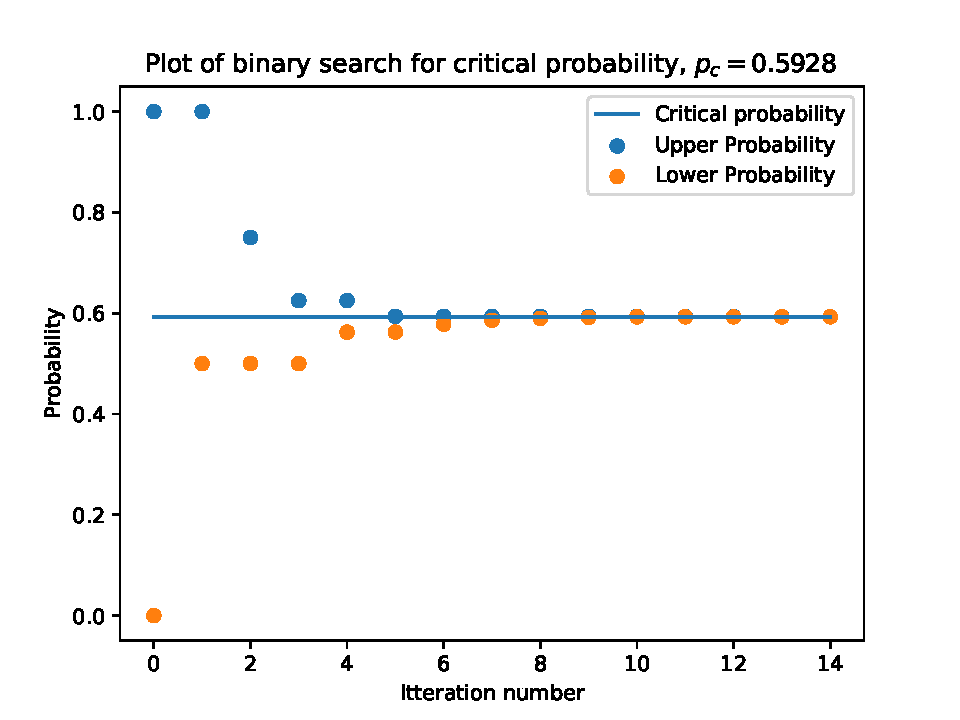
\includegraphics[width=\linewidth]{report/assets/critical_prob.pdf}
    \caption{Convergence of binary search for critical probability in 2d site percolation, for a square grid with side length 40,000}
\end{figure}
\begin{itemize}
\item number of clusters
\item Give reasoning for shape of the curve at three values of p
\item Link into polyminoes
\item polyminoes
\begin{itemize}
\item What is a polymino
\end{itemize}
\item critical probability
\begin{itemize}
\item Show results from critical probability 
\item  Introduce plots
\item  Identify critical point on graph
\item Calculate critical exponents from graph
\end{itemize}
\item  Weird graph?
\begin{itemize}
\item Understand what's going on physically
\item Describe why this may be of importance
\end{itemize}
\end{itemize}

\subsection{FF}
\begin{itemize}
\item Gifs
\end{itemize}

\section{Discussion}

\section{Conclusion}

\bibliography{apssamp}% Produces the bibliography via BibTeX.

\end{document}
%
% ****** End of file apssamp.tex ******
